\section{Chain Complexes}
\label{sec:Chain Complexes}
\begin{definition}
	A chain complex $C$ is a collection of abelian groups $C_n$ together with boundary operators $\del_n: C_{n+1} \to C_n$, such that $\del_n \circ \del_{n+1} = 0$. The collections of all such objects will be denoted by $\Ch{\cat{Ab}}$.
\end{definition}

In other words a chain complex is the following diagram.
$$ \cdots \to C_4 \to C_3 \to C_2 \to C_1 \to C_0 $$

Of course we can make this more general by taking for example $R$-modules instead of abelian groups. We will later see which kind of algebraic objects make sense to use in this definition. The boundary operators give rise to certain subgroups, because all groups are abelian, subgroups are normal subgroups.

\begin{definition}
	Given a chain complex $C$ we define the following subgroups:
	\begin{itemize}
		\item $Z_n(C) = ker(\del: C_n \to C_{n-1}) \nsubgrp C_n$, and
		\item $B_n(C) = im(\del: C_{n+1} \to C_n) \nsubgrp C_n$.
	\end{itemize}
\end{definition}
\begin{lemma}
	Given a chain complex $C$ we have for all $n \in \N$:
	$$ B_n(C) \nsubgrp Z_n(C).$$
\end{lemma}
\begin{proof}
	It follows from $\del_n \circ \del_{n+1} = 0$ that $im(\del: C_{n+1} \to C_n)$ is a subset of $ker(\del: C_n \to C_{n-1})$. Those are exactly the abelian groups $B_n(C)$ and $Z_n(C)$, so $ B_n(C) \nsubgrp Z_n(C) $.
\end{proof}
\begin{definition}
	Given a chain complex $C$ we define the \emph{$n$-th homology group} $H_n(C)$:
	$$ H_n(C) = Z_n(C) / B_n(C).$$
\end{definition}

\subsection{The singular chain complex}
In order to see why we are interested in the construction of homology groups, we will look at an example from algebraic topology. We will see that homology gives a nice invariant for spaces. So we will form a chain complex from a topological space $X$. In order to do so, we first need some more notions.
\begin{definition}
	The topological space $\Delta^n$ is called the \emph{topological $n$-simplex} and is defined as:
	$$ \Delta^n = \{x \in \R^{n+1} \I x_i \geq 0 \text{ and } x_0 + \ldots + x_n = 1 \}.$$
	The topology on $\Delta^n$ is the subspace topology.
\end{definition}

In particular $\Delta^0$ is simply a point, $\Delta^1$ a line and $\Delta^2$ a triangle. There are nice inclusions $\Delta^n \inject \Delta^{n+1}$ which we need later on. For any $n \in \N$ we define:
\begin{definition}
	For $i \in \{0, \ldots, n+1\}$ the $i$-th face map $\delta^i : \Delta^n \inject \Delta^{n+1}$ is defined as:
	$$ \delta^i (x_0, \ldots, x_n) = (x_0, \ldots, x_{i-1}, 0, x_{i+1}, \ldots, x_n) \text{ for all } x \in \Delta^n.$$
\end{definition}

Note that if we have any continuous map $\sigma : \Delta^{n+1} \to X$ we can precompose with a face map to get $\sigma \circ \delta^i : \Delta^n \to X$. This will be used for defining the boundary operator. We can make pictures of this, and when concerning continuous maps $\sigma : \Delta^{n+1} \to X$ we will draw the images in the space $X$, instead of functions.

\todo{Ch: Make some pictures here}

\todo{Ch: Define free abelian group}

We now have enough tools to define the singular chain complex of a space $X$.

\begin{definition}
	For a topological space $X$ we define an abelian group $C_n(X)$ as follows.
	$$ C_n(X) = \Z[\Hom{\cat{Top}}{\Delta^n}{X}] $$
	The boundary operator $\del : C_{n+1}(X) \to C_n(X)$ is defined on generators as:
	$$ \del(\sigma) = \sigma \circ \delta^0 - \sigma \circ \delta^1 + \ldots + (-1)^{n+1} \sigma \circ \delta^{n+1}.$$
\end{definition}

This might seem a bit complicated, but we can pictures this in an intuitive way, as in figure~\ref{fig:singular_chaincomplex3}. And we see that the boundary operators really give the boundary of an $n$-simplex. To see that this indeed is a chain complex we have to proof that the composition of two such operators is the zero map.
\begin{figure}
	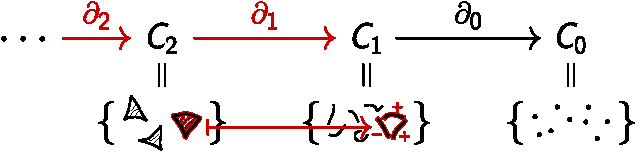
\includegraphics{singular_chaincomplex3}
	\caption{The boundary of a 2-simplex}
	\label{fig:singular_chaincomplex3}
\end{figure}

\todo{Ch: Proposition: $C(X) \in \Ch{\cat{Ab}}$}

\todo{Ch: Example homology of some space}

\todo{Ch: Show that $\Ch{\Ab}$ is an ab. cat. At least show functoriality $\Hom{\Ch{\Ab}}{-}{-}$}
